\section{Entropy}\label{sec:Entropy}
\subsection{Clausius Inequality}\label{subsec:Clausius_Inequality}
We have 2 equations for the efficiency of a \nameref{def:Carnot_Cycle}.
\begin{align*}
  \Efficiency_{\text{Carnot}} &= \frac{\Temp_{H} - \Temp_{L}}{\Temp_{H}} = 1 - \frac{\Temp_{L}}{\Temp_{H}} \\
                              &= \frac{\Heat_{H} - \Heat_{L}}{\Heat_{H}} = 1 - \frac{\Heat_{L}}{\Heat_{H}}
\end{align*}

\subsubsection{Reversible Carnot Cycles}\label{subsubsec:Reversible_Carnot_Cycles}
If we equate these (set them equal to each other) we get:
\begin{align*}
  1 - \frac{\Temp_{L}}{\Temp_{H}} &= 1 - \frac{\Heat_{L}}{\Heat_{H}} \\
  \frac{\Temp_{L}}{\Temp_{H}} &= \frac{\Heat_{L}}{\Heat_{H}} \\
  \frac{\Heat_{L}}{\Temp_{L}} &= \frac{\Heat_{H}}{\Temp_{H}} \\
  \frac{\Heat_{L}}{\Temp_{L}} - \frac{\Heat_{H}}{\Temp_{H}} &= 0
\end{align*}

This derivation's result is valid for any \nameref{def:Reversible_Process} which is a \nameref{def:Carnot_Cycle}.

\subsubsection{Irreversible Carnot Cycles}\label{subsubsec:Irreversible_Carnot_Cycles}
Looking at the energy balance present for an \nameref{def:Irreversible_Process}
\begin{equation*}
  \Heat_{H} - \Heat_{L} = \Work_{Out} + \Work_{\text{Friction}}
\end{equation*}

Because of the presence of $\Work_{\text{Friction}}$, $\Heat_{L}$ gets smaller (in comparison to a reversible Carnot cycle).
That means that the heat/temperature ratio equation has changed.
\begin{equation*}
  \frac{\Heat_{L}}{\Temp_{L}} - \frac{\Heat_{H}}{\Temp_{H}} < 0
\end{equation*}

Here, we start getting into the topic of \nameref{def:Entropy} a little bit more.

\begin{equation}\label{eq:Clausius_Inequality}
  \sum\limits_{i} \frac{d \Heat_{i}}{\Temp_{i}} \leq 0
\end{equation}

There are some things to say about \Cref{eq:Clausius_Inequality}.
\begin{itemize}[noitemsep]
\item Assume that you know the directions for the heats.
\item The $\frac{d \Heat_{i}}{\Temp_{i}}$ is called \nameref{def:Entropy}, or $\Entropy$.
\item If we divide the \nameref{def:Entropy} by the mass, we have the \nameref{def:Specific_Entropy}, $\frac{\frac{d \Heat_{i}}{\Temp_{i}}}{\Mass}$.
\end{itemize}

\subsubsection{Heat Engines and the Clausius Inequality}\label{subsubsec:Heat_Engine_Clausius_Inequality}
If we imagine a heat engine running through a set of cycles, as shown in \Cref{fig:Heat_Engine_Clausius_Inequality}, then we can say some things about it.

\begin{figure}[h!tbp]
  \centering
  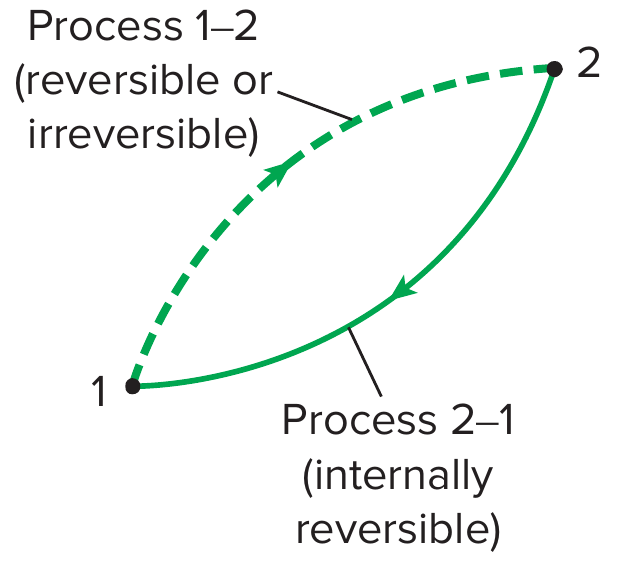
\includegraphics[scale=0.35]{Heat_Engine_Clausius_Inequality.png}
  \caption{Heat Engines and the Clausius Inequality (\cite[pg. 280]{ThermoTextbook})}
  \label{fig:Heat_Engine_Clausius_Inequality}
\end{figure}

Namely, the thing we can say is:
\begin{align*}
  \int\limits_{1}^{2} \frac{d \Heat}{\Temp} + \int\limits_{2}^{1} \frac{d \Heat}{\Temp} &\leq 0 \\
  \int\limits_{1}^{2} \Entropy + \int\limits_{2}^{1} \Entropy &\leq 0 \\
  (\Entropy_{1} - \Entropy_{2}) + \int\limits_{2}^{1} \Entropy &\leq 0 \\
  \Entropy_{2} - \Entropy_{1} &\geq \int\limits_{2}^{1} \frac{d \Heat}{\Temp}
\end{align*}

This last point is actually quite important and is restated here.
\begin{equation}\label{eq:Reversible_Process_Entropy_Lost}
  \Entropy_{2} - \Entropy_{1} \geq \int\limits_{2}^{1} \frac{d \Heat}{\Temp}
\end{equation}

\Cref{eq:Reversible_Process_Entropy_Lost} states that for an \nameref{def:Irreversible_Process}, \nameref{def:Work} is lost \textbf{forever}.
\begin{itemize}[noitemsep]
\item For \nameref{def:Irreversible_Process}es, $\Entropy$ \textbf{always} increases.
\item For \nameref{def:Reversible_Process}es, $\Change{\Entropy} = 0$.
\end{itemize}

%%% Local Variables:
%%% mode: latex
%%% TeX-master: "../../MMAE_320-Thermo-Reference_Sheet"
%%% End:


\subsubsection{Entropy and its Definitions}\label{subsec:Entropy_Definitions}
\begin{definition}[Entropy]\label{def:Entropy}
  \emph{Entropy} is an thermodynamically \nameref{def:Extensive_Property}.
  It is defined from the \nameref{subsec:Clausius_Inequality}, in \Cref{eq:Clausius_Inequality}.
  \begin{equation}\label{eq:Entropy}
    \Entropy = \frac{\Heat_{i}}{\Temp_{i}}
  \end{equation}

  Another equation to describe entropy is based on the concept of the number of energy states.
  \begin{equation}\label{eq:Entropy_Energy_States}
    \Entropy = \BoltzmannConstant \ln(W)
  \end{equation}
  where:
  \begin{description}[noitemsep]
  \item $\BoltzmannConstant$ is Boltzmann's Constant.
  \item $W$ is the number of energy states in the system.
    This value is usually proportional to temperature or some energy.
  \end{description}
\end{definition}

\begin{definition}[Specific Entropy]\label{def:Specific_Entropy}
  \emph{Specific Entropy}, like all the other specific properties of a state, is a thermodynamically \nameref{def:Intensive_Property}.
  Similarly to \nameref{def:Entropy}, specific entropy is defined from the \nameref{subsec:Clausius_Inequality}, in \Cref{eq:Clausius_Inequality}, but is also divided by the mass.
  \begin{equation}\label{eq:Entropy}
    \SpecificEntropy = \frac{\frac{\Heat_{i}}{\Temp_{i}}}{\Mass}
  \end{equation}
\end{definition}

There also exist \nameref{def:Cycle}s where the \nameref{def:Entropy} remains constant (which only happens if the \nameref{def:Process} is a \nameref{def:Reversible_Process}), which are called \nameref{def:Isentropic}.
These can only occur if the \nameref{def:Process} is \nameref{def:Adiabatic}.

\begin{definition}[Isentropic]\label{def:Isentropic}
  An \emph{isentropic} \nameref{def:Process}/\nameref{def:Cycle} has constant \nameref{def:Entropy}.
\end{definition}

\begin{example}[Textbook Problem 8.38]{Isentropic Ideal Gases}
  $\Mass = \SI{1}{\lbm}$ R-134a is expanded \nameref{def:Isentropic}ly in a \nameref{def:Closed_System} that goes from $\Pressure_{1} = \SI{100}{\psia}$ and $\Temp_{1} = \SI{100}{\degreeF}$ to $\Pressure_{2} = \SI{10}{\psia}$.
  Determine the total heat transfer and the work required for this \nameref{def:Process}?
  \tcblower{}
  \textbf{Concepts:} \\
  This is a \nameref{def:Closed_System}, so mass is constant, there is \textbf{no} mass flow.
  However, there can still be a heat and work flow. \\
  We are told this is an \nameref{def:Isentropic} process, so there is no change in temperature.
  \begin{align*}
    \Temp_{1} &= \Temp_{2} \\
    \Change{\Entropy} &= 0 \\
    \frac{\Change{\Heat}}{\Temp} &= 0 \\
    \Change{\Heat} &= 0
  \end{align*}

  There is a change in pressure, meaning the vessel itself expands.

  \textbf{Explore:} \\
  Pressure is \textbf{not} constant. \\
  The vessel is expanding, meaning there needs to be a change in energy.
  The energy is coming from the internal energy, $\InternalEnergy$, of the gas because the R-134a is not ``pushing'' against anything. \\
  We discovered that $\Change{\Heat} = 0$. \\
  We are not told about any work in, so assume $\Work_{In} = 0$.

  The energy balance is now:
  \begin{equation*}
    -\Work_{Out} = \Mass (\SpecificInternalEnergy_{2} - \SpecificInternalEnergy_{1}) \\
  \end{equation*}

  We can use Tables A.11E through A.13E to find values for R-134a.

  \textbf{Plan:} \\
  Using the pressures and temperatures, use the Tables to find the entropies and the internal energies.
  Remember that $\SpecificEntropy_{1} = \SpecificEntropy_{2}$, so we can find the different internal energies.

  \textbf{Solve:} \\
  Start by using Table A.13E at $\Pressure_{1} = \SI{100}{\psia}$ and $\Temp_{1} = \SI{100}{\degreeF}$ to find the initial properties of the R-134a.
  \begin{align*}
    \SpecificEntropy_{1} &= \SI{0.22902}{\btu\per\lbm\per\rankine} \\
    \SpecificInternalEnergy_{1} &= \SI{109.46}{\btu\per\lbm}
  \end{align*}

  Now, using the facts that $\SpecificEntropy_{1} = \SpecificEntropy_{2}$, and $\Pressure_{2} = \SI{10}{\psia}$, we use Table A.13E again, looking for a $\SpecificEntropy_{2}$ that is as similar to $\SpecificEntropy_{1}$ as possible.
  \begin{align*}
    \SpecificEntropy_{2} &= \SI{0.22949}{\btu\per\lbm\per\rankine} \\
    \Temp_{2} &= \SI{-29.52}{\degreeF} \\
    \SpecificInternalEnergy_{2} &= \SI{113.02}{\btu\per\lbm}
  \end{align*}

  \textbf{Validate:} \\

  \textbf{Generalize:} \\

\end{example}

\subsection{Isentropic Efficiencies}\label{subsec:Isentropic_Efficiencies}
Consider a \nameref{fig:Heat_Engine}, like the one shown in \Cref{fig:Heat_Engine}.
\begin{itemize}[noitemsep]
\item If each sub-\nameref{def:Process} is \nameref{def:Isentropic}, then on a $\Temp-\Entropy$ graph, then the process is perfectly vertical.
\item If any part is even slightly irreversible, then the ending entropy is further to the right compared ot any previous part of the \nameref{def:Cycle}.
\end{itemize}

If we are talking in a non-ideal case, then we can say:
\begin{equation*}
  \Efficiency = \frac{\Work_{Out}}{\Heat_{In}}
\end{equation*}

\subsubsection{Turbine}\label{subsubsec:Turbine_Isentropic_Efficiency}
If we deal with the actual work out and ideal heat in, we say the \nameref{def:Isentropic} efficiency is:
\begin{align*}
  \Isentropic{\Efficiency} &= \frac{\Work_{Out, \text{Actual}}}{\Heat_{In, \text{Ideal}}} \\
                           &= \frac{\FlowRate{\Mass}(\SpecificEnthalpy_{In} - \SpecificEnthalpy_{Out, \text{Actual}})}{\FlowRate{\Mass} (\SpecificEnthalpy_{In} - \SpecificEnthalpy_{Out, \text{Ideal}})} \\
                           &= \frac{\SpecificEnthalpy_{In} - \SpecificEnthalpy_{Out, \text{Actual}}}{\SpecificEnthalpy_{In} - \SpecificEnthalpy_{Out, \text{Ideal}}}
\end{align*}

For a \nameref{def:Turbine},
\begin{equation}\label{eq:Isentropic_Efficiency-Turbine}
  \Isentropic{\Efficiency} = \frac{\SpecificEnthalpy_{In} - \SpecificEnthalpy_{Out, \text{Actual}}}{\SpecificEnthalpy_{In} - \SpecificEnthalpy_{Out, \text{Ideal}}}
\end{equation}

\begin{example}{Turbine Entropy}
  Given an \nameref{def:Adiabatic} \nameref{def:Turbine} that uses steam where the inlet steam is at $\Pressure_{In} = \SI{1000}{\psia}$ and $\Temp_{In} = \SI{800}{\degreeF}$.
  The outlet is $\Pressure_{Out} = \SI{400}{\psia}$.
  Find $\frac{\FlowRate{\Work_{Out}}}{\FlowRate{\Mass}}$?
  \tcblower{}
  \textbf{Concepts:} \\
  This is a \nameref{def:Turbine}, so it has constant flow.
  Meaning $\FlowRate{\Mass}_{In} = \FlowRate{\Mass}_{Out}$. \\
  This is an \nameref{def:Adiabatic} \nameref{def:Turbine}, which means the \nameref{def:Process} is a \nameref{def:Reversible_Process}, and is an \nameref{def:Isentropic} process.
  Meaning $\SpecificEntropy_{In} = \SpecificEntropy_{Out}$. \\
  Lastly, energy is conserved, so $\FlowRate{\Energy}_{In} = \FlowRate{\Energy}_{Out}$.

  \textbf{Explore:} \\
  The change in energy is due to the \nameref{def:Enthalpy} changes in the steam. \\
  The \nameref{def:Specific_Entropy} remains unchanged throughout the process, so we can use these values from Tables. \\
  Tables A.4E --- A.7E will help us solve this.

  \textbf{Plan:} \\
  Find the steam's initial state properties, $\SpecificEnthalpy_{In}$ and $\SpecificEntropy_{In}$. \\
  Use $\SpecificEntropy_{In} = \SpecificEntropy_{Out}$ to help find $\SpecificEnthalpy_{Out}$. \\
  Use the energy balance equation for a \nameref{def:Turbine} $\FlowRate{\Work}_{Out} = \FlowRate{\Mass}(\SpecificEnthalpy_{Out} - \SpecificEnthalpy_{In})$ and solve for $\frac{\FlowRate{\Work_{Out}}}{\FlowRate{\Mass}}$.

  \textbf{Solve:} \\
  The steam enters the \nameref{def:Turbine} as a \nameref{def:Superheated_Vapor}, so we use Table A.6E.
  From Table A.6E at $\Pressure_{In} = \SI{1000}{\psia}$ and $\Temp_{In} = \SI{800}{\degreeF}$, we see:
  \begin{description}[noitemsep]
  \item $\SpecificEnthalpy_{In} = \SI{1389.0}{\btu\per\lbm}$
  \item $\SpecificEntropy_{In} = \SI{1.5670}{\btu\per\lbm\per\rankine}$
  \end{description}

  Now, for the outlet state.
  Start by looking at Table A.5E at $\Pressure_{Out} = \SI{400}{\psia}$.
  If we look at the \nameref{def:Specific_Entropy} entries, we see that the highest value is when the steam is a \nameref{def:Saturated_Vapor}, with $\Vapor{\SpecificEntropy} = \SI{1.4852}{\btu\per\lbm\per\rankine}$.
  However, because $\SpecificEntropy_{In} = \SpecificEntropy_{Out}$, we see that this is not enough.
  So, that means the steam is still a \nameref{def:Superheated_Vapor} at the outlet. \\
  From Table A.6E, at $\Pressure_{Out} = \SI{400}{\psia}$, we look for $\SpecificEntropy_{Out} = \SI{1.5670}{\btu\per\lbm\per\rankine}$.
  The closest value to that $\SpecificEntropy$ is at $\Temp_{Out} = \SI{550}{\degreeF}$, with $\SpecificEnthalpy_{Out} = \SI{1277.3}{\btu\per\lbm}$.
  (In reality, we should \nameref{def:Interpolate} our values, but this is close enough for this example.)

  Now, solving the energy balance equation for $\frac{\FlowRate{\Work}_{Out}}{\FlowRate{\Mass}}$.
  \begin{align*}
    - \FlowRate{\Work}_{Out} &= \FlowRate{\Mass} (\SpecificEnthalpy_{Out} - \SpecificEnthalpy_{In}) \\
    \frac{-\FlowRate{\Work}_{Out}}{\FlowRate{\Mass}} &= \SpecificEnthalpy_{Out} - \SpecificEnthalpy_{In} \\
    \frac{\FlowRate{\Work}_{Out}}{\FlowRate{\Mass}} &= \SpecificEnthalpy_{In} - \SpecificEnthalpy_{Out} \\
                           &= \SI{1389.0}{\btu\per\lbm} - \SI{1277.3}{\btu\per\lbm} \\
    &= \SI{111.7}{\btu\per\lbm}
  \end{align*}

  \textbf{Generalize:} \\
  We can use \nameref{def:Specific_Entropy} to find the state of the working fluid, just like the \nameref{def:Specific_Enthalpy}, temperature, or pressure.
\end{example}

\begin{example}[Textbook Example 8.14]{Isentropic Efficiency of a Steam Turbine}
  Steam enters an \nameref{def:Adiabatic} \nameref{def:Turbine} steadily at $\Pressure_{In} = \SI{3}{\mega\pascal}$ and $\Temp_{In} = \SI{400}{\degreeCelsius}$ and leaves at $\Pressure_{Out} = \SI{50}{\kilo\pascal}$ and $\Temp_{Out} = \SI{100}{\degreeCelsius}$.
  If the power output of the turbine is $\FlowRate{\Work}_{Out}= \SI{2}{\mega\watt}$, determine the isentropic efficiency of the turbine and the mass flowrate of the steam flowing through the turbine?
  \tcblower{}
  \textbf{Concepts:} \\
  We are given the information for both the inlet and the outlet.
  These are the actual values of the turbine.
  If we want the idealized values, we need to interpret the inlet data a little bit. \\
  For a turbine be \nameref{def:Isentropic}, it needs to be \nameref{def:Adiabatic}, which we are told it is.
  This means that $\SpecificEntropy_{In} = \SpecificEntropy_{Out}$. \\
  The isentropic efficiency of a turbine is seen in \Cref{eq:Isentropic_Efficiency-Turbine}.

  \textbf{Explore:} \\
  Because this is steam, Tables A.4 through A.7 will be of use. \\
  The idealized values for the ideal case can only be found by treating this system as \nameref{def:Adiabatic} and ensuring that $\SpecificEntropy_{In} = \SpecificEntropy_{Out}$.

  \textbf{Plan:} \\
  Use the tables to find the actual inlet and outlet specific enthalpies. \\
  Use the idea that $\SpecificEntropy_{In} = \SpecificEntropy_{Out}$ to find the ideal outlet specific enthalpy. \\
  Solve \Cref{eq:Isentropic_Efficiency-Turbine} for $\Isentropic{\Efficiency}$.
\end{example}

\begin{example}[Textbook Problem 8.128]{Power Output of Isentropically Efficienct Steam Turbine}
  Steam at $\Pressure_{In} = \SI{3}{\mega\pascal}$ and $\Temp_{In} = \SI{400}{\degreeCelsius}$ is expanded to $\Pressure_{Out} = \SI{30}{\kilo\pascal}$ in an \nameref{def:Adiabatic} \nameref{def:Turbine} with an \nameref{def:Isentropic} efficiency of $\Isentropic{\Efficiency} = 0.92$.
  Determine the power produced by this turbine ($\FlowRate{\Work}_{Out}$) in \si{\kilo\watt} when the mass flowrate is $\FlowRate{\Mass} = \SI{2}{\kilo\gram\per\second}$?
  \tcblower{}
  \textbf{Concepts:} \\
  This is a \nameref{def:Turbine}, with \nameref{def:Adiabatic} steady flow.
  A turbine gets all its energy from the change in \nameref{def:Enthalpy}, $\Change{\SpecificEnthalpy}$. \\
  The equation for \nameref{def:Isentropic} efficiency is:
  \begin{equation*}
    \Isentropic{\Efficiency} = \frac{\text{Actual Work Out}}{\text{Isentropic Work Out}}
  \end{equation*}

  \textbf{Explore:} \\
  To solve for the work out, we need to know the maximum work out that we could gather.
  This only occurs if the \nameref{def:Turbine} is perfectly \nameref{def:Isentropic}, meaning $\Entropy_{In} = \Entropy_{Out}$.

  If we expand the isentropic efficiency equation, then we get:
  \begin{equation*}
    \Isentropic{\Efficiency} = \frac{\SpecificEnthalpy_{In} - \SpecificEnthalpy_{Out, \text{Actual}}}{\SpecificEnthalpy_{In} - \SpecificEnthalpy_{Out, \text{Ideal}}}
  \end{equation*}

  The energy balance for this turbine is:
  \begin{equation*}
    \FlowRate{\Work}_{Out, \text{Actual}} = \FlowRate{\Mass} (\SpecificEnthalpy_{In} - \SpecificEnthalpy_{Out})
  \end{equation*}

  This is a steam turbine, so Tables A.4 through A.7 will be of use.

  \textbf{Plan:} \\
  Find properties of the initial state, $\SpecificEnthalpy_{In}$, $\SpecificEntropy_{In}$. \\
  Use our assumption of isentropic to find $\SpecificEntropy_{Out, \text{Ideal}}$.

  \textbf{Solve:} \\
  We see that from the inlet fluid's pressure and temperature, it is a \nameref{def:Superheated_Vapor}, so we use Table A.6.
  From Table A.6 at $\Pressure_{In} = \SI{3}{\mega\pascal}$ and $\Temp_{In} = \SI{400}{\degreeCelsius}$, we have:
  \begin{align*}
    \SpecificEnthalpy_{In} &= \SI{3231}{\kilo\joule\per\kilo\gram} \\
    \SpecificEntropy_{In} &= \SI{6.923}{\kilo\joule\per\kilo\gram\per\kelvin}
  \end{align*}

  If we assume that the \nameref{def:Turbine} is perfectly \nameref{def:Isentropic}, then we notice that the steam has become a \nameref{def:Saturated_Mixture}, so we use Table A.5 to find its properties.
  \begin{align*}
    \Quality &= \frac{\SpecificEntropy_{In} - \Fluid{\SpecificEntropy}}{\Vapor{\SpecificEntropy} - \Fluid{\SpecificEntropy}} \\
             &= \frac{6.923 - 0.9441}{7.7675 - 0.9441} \\
    \Quality &= 0.8763
  \end{align*}

  Now, we find the ideal $\SpecificEnthalpy_{Out, \text{Ideal}}$.
  \begin{align*}
    \SpecificEnthalpy_{Out, \text{Ideal}} &= \Fluid{\SpecificEnthalpy} + \Quality (\Vapor{\SpecificEnthalpy} - \Fluid{\SpecificEnthalpy}) \\
                                          &= 289.27 + 0.8763 (2624.6 - 289.27) \\
                                          &= \SI{2335.72}{\kilo\joule\per\kilo\gram}
  \end{align*}

  So, the \nameref{def:Isentropic} work out is:
  \begin{align*}
    \FlowRate{\Work}_{Out, \text{Ideal}} &= \FlowRate{\Mass} (\SpecificEnthalpy_{In} - \SpecificEnthalpy_{Out, \text{Ideal}}) \\
                                         &= 2 (3231 - 2335.72) \\
                                         &= \SI{1790.56}{\kilo\joule\per\second}
  \end{align*}

  Now, we plug that into our isentropic efficiency.
  \begin{align*}
    \Isentropic{\Efficiency} &= \frac{\FlowRate{\Work}_{Out, \text{Actual}}}{\FlowRate{\Work}_{Out, \text{Ideal}}} \\
    \shortintertext{Rearranging the equation.}
    \FlowRate{\Work}_{Out, \text{Actual}} &= \Isentropic{\Efficiency} \FlowRate{\Work}_{Out, \text{Ideal}} \\
                             &= 0.92 (1790.56) \\
                             &= \SI{1647.32}{\kilo\joule\per\second}
  \end{align*}

  \textbf{Validate:} \\

  \textbf{Generalize:} \\

\end{example}

\subsubsection{Compressor}\label{subsubsec:Compressor_Isentropic_Efficiency}
For a \nameref{def:Compressor}, we have:
\begin{equation}\label{eq:Isentropic_Efficiency-Compressor}
  \begin{aligned}
    \Isentropic{\Efficiency} &= \frac{\text{\nameref{def:Isentropic} Work In}}{\text{Actual Work In}} \\
    &= \frac{\SpecificEnthalpy_{Out, \text{Ideal}} - \SpecificEnthalpy_{In}}{\SpecificEnthalpy_{Out, \text{Actual}} - \SpecificEnthalpy_{In}}
  \end{aligned}
\end{equation}

\begin{example}[Textbook Problem 8.24]{Isentropic Compressor}
  Air is compressed by a $\FlowRate{\Work}_{In} = \SI{12}{\kilo\watt}$ \nameref{def:Compressor}.
  The air temperature is maintained at $\Temp = \SI{25}{\degreeCelsius}$ during the process.
  Then, as a result of \nameref{def:Heat_Transfer}, the surrounding air, which is at $\Temp = \SI{10}{\degreeCelsius}$.
  Determine the rate of entropy change of the air?
  \tcblower{}
  \textbf{Concepts:} \\
  \nameref{def:Compressor}s typically increase the air's temperature.
  Because there is no temperature change of the air, that means the whole compressor is being cooled, thus a $\FlowRate{\Heat}_{Out} \neq 0$. \\
  We find the $\FlowRate{\Entropy}$, but we aren't given a mass flowrate, $\FlowRate{\Mass}$. \\
  We should also treat air as an ideal gas.

  \textbf{Explore:} \\
  We can ignore $\PotentialEnergy$ and $\KineticEnergy$.
  The energy balance for a compressor is:
  \begin{equation*}
    \FlowRate{\Work}_{In} - \FlowRate{\Heat}_{Out} = \FlowRate{\Mass} (\SpecificEnthalpy_{Out} - \SpecificEnthalpy_{In})
  \end{equation*}

  Inside the \nameref{def:Compressor}, it is \nameref{def:Isothermal}.
  Therefore, the \nameref{def:Process} \textbf{INSIDE} the compressor is a \nameref{def:Reversible_Process}, so it is \nameref{def:Isentropic}. \\
  Using the energy balance $\FlowRate{\Energy}_{In} = \FlowRate{\Energy}_{Out}$, we can say:
  \begin{align*}
    \FlowRate{\Energy}_{In} &= \FlowRate{\Energy}_{Out} \\
    \FlowRate{\Work}_{In} + \FlowRate{\Mass} \SpecificEnthalpy_{In} &= \FlowRate{\Heat}_{Out} + \FlowRate{\Mass} \SpecificEnthalpy_{Out} \\
    \intertext{Because $\SpecificEnthalpy \propto \Temp$, substitute for temperatures.
    We can do this because of the specific enthalpy-specific heat equations for ideal gases.}
    \FlowRate{\Work}_{In} + \FlowRate{\Mass} \Temp_{In} &= \FlowRate{\Heat}_{Out} + \FlowRate{\Mass} \Temp_{In} \\
    \intertext{And, the temperatures are the same, so they cancel out.}
    \FlowRate{\Work}_{In} &= \FlowRate{\Heat}_{Out}
  \end{align*}

  Lastly, we can find the \nameref{def:Entropy} flowrate.
  \begin{align*}
    \Entropy &= \frac{\Heat}{\Temp} \\
    \FlowRate{\Entropy} &= \frac{\FlowRate{\Heat}}{\Temp} \\
    \intertext{Because the heat is flowing outwards, there is actually a negative.}
    \FlowRate{\Entropy} &= \frac{-\FlowRate{\Heat}}{\Temp}
  \end{align*}

  \textbf{Plan:} \\
  Solve for the entropy flowrate, $\FlowRate{\Entropy}$.

  \textbf{Solve:} \\
  \begin{align*}
    \FlowRate{\Entropy} &= \frac{-\FlowRate{\Heat}}{\Temp} \\
                        &= \frac{\SI{-12}{\kilo\watt}}{(25 + 273.15)\si{\kelvin}} \\
                        &= \SI{-0.0403}{\kilo\watt\per\kelvin}
  \end{align*}

  \textbf{Validate:} \\
  Even though the \nameref{def:Entropy} inside the system decreased, the overall entropy of the entire system (compressor and surroundings) increased by a similar amount.
  \begin{align*}
    \FlowRate{\Entropy} &= \frac{\FlowRate{\Heat}}{\Temp} \\
                        &= \frac{\SI{12}{\kilo\watt}}{(10 + 273.15)\si{\kelvin}} \\
                        &= \SI{0.0424}{\kilo\watt\per\kelvin}
  \end{align*}

  \textbf{Generalize:} \\
  If we add the entropy gained by the surroundings and the entropy lost by the \nameref{def:Compressor} together, we get a non-zero result.
  This aligns with what we understand about \nameref{def:Entropy} and \nameref{def:Irreversible_Process}es and the fact that we assumed this process was actually a \nameref{def:Reversible_Process}.
\end{example}

\begin{example}[Textbook Problem 8.130]{Isentropic Efficiency of Compressor}
  An \nameref{def:Adiabatic} steady-flow device compresses argon at $\Pressure_{In} = \SI{200}{\kilo\pascal}$ and $\Temp_{In} = \SI{27}{\degreeCelsius}$ to $\Pressure_{Out} = \SI{2}{\mega\pascal}$.
  If the argon leaves this \nameref{def:Compressor} at $\Temp_{Out} = \SI{550}{\degreeCelsius}$ what is the isentropic efficiency, $\Isentropic{\Efficiency}$ of the compressor?
  \tcblower{}
  \textbf{Concepts:} \\
  Because the working fluid is argon, it is an ideal gas.
  The equations we found for ideal gases are really just approximations.
  We have $\SpecificHeatPressure$, $\SpecificHeatVolume$, and $k$. \\
  Since we need to assume that the system is \nameref{def:Isentropic} for some of the calculations, we have some equations that we can use for an ideal gas (\Cref{subsec:Ideal_Gases_Entropy_Changes}).

  \textbf{Explore:} \\
  The efficiency of a compressor is:
  \begin{equation*}
    \Isentropic{\Efficiency} = \frac{\FlowRate{\Work}_{In, \text{Ideal}}}{\FlowRate{\Work}_{Out, \text{Actual}}}
  \end{equation*}

  The energy balance for a compressor is:
  \begin{equation*}
    \FlowRate{\Work}_{In} = \FlowRate{\Mass} (\SpecificEnthalpy_{Out} - \SpecificEnthalpy_{In})
  \end{equation*}

  If we substitute that into the isentropic efficiency equation:
  \begin{align*}
    \Isentropic{\Efficiency} &= \frac{\FlowRate{\Work}_{In, \text{Ideal}}}{\FlowRate{\Work}_{Out, \text{Actual}}} \\
                             &= \frac{\FlowRate{\Mass} (\SpecificEnthalpy_{Out, \text{Ideal}} - \SpecificEnthalpy_{In})}{\FlowRate{\Mass} (\SpecificEnthalpy_{Out, \text{Actual}} - \SpecificEnthalpy_{In})} \\
    \shortintertext{We can cancel out like terms.}
                             &= \frac{\Change{\SpecificEnthalpy}_{\text{Ideal}}}{\Change{\SpecificEnthalpy}_{\text{Actual}}} \\
    \intertext{Because this is an ideal gas, we can substitute in \Cref{eq:Change_Internal_Energy_Specific_Heat_Constant_Pressure}.}
                             &= \frac{\SpecificHeatPressure \Change{\Temp}_{\text{Ideal}}}{\SpecificHeatPressure \Change{\Temp}_{\text{Actual}}} \\
                             &\approx \frac{\Change{\Temp}_{\text{Ideal}}}{\Change{\Temp}_{\text{Actual}}} \\
    &= \frac{\Temp_{Out, \text{Ideal}} - \Temp_{In}}{\Temp_{Out, \text{Actual}} - \Temp_{In}}
  \end{align*}

  To find the \nameref{def:Isentropic} output fluid temperature, we have \Crefrange{subeq:Isentropic_Ideal_Gas-Pressure_Volume}{subeq:Isentropic_Ideal_Gas-Temperature_Pressure}.
  \begin{align*}
    \frac{\Temp_{2}}{\Temp_{1}} &= {\left( \frac{\Pressure_{2}}{\Pressure_{1}} \right)}^{\frac{k-1}{k}} \\
    \Temp_{Out, \text{Ideal}} &= \Temp_{In} {\left( \frac{\Pressure_{2}}{\Pressure_{1}} \right)}^{\frac{k-1}{k}}
  \end{align*}
  where $k = \frac{\SpecificHeatPressure}{\SpecificHeatVolume}$.

  Table A.2 will have these values.

  \textbf{Plan:} \\
  Solve for the \nameref{def:Isentropic} output fluid temperature.

  \textbf{Solve:} \\
  From Table A.2:
  \begin{align*}
    \SpecificHeatPressure &= \SI{0.5203}{\kilo\joule\per\kilo\gram\per\kelvin} \\
    \SpecificHeatVolume &= \SI{0.3122}{\kilo\joule\per\kilo\gram\per\kelvin} \\
    k &= 1.667
  \end{align*}

  Solving for the ideal outlet fluid temperature:
  \begin{align*}
    \Temp_{Out, \text{Ideal}} &= \Temp_{In} {\left( \frac{\Pressure_{2}}{\Pressure_{1}} \right)}^{\frac{k-1}{k}} \\
                              &= (27 + 273.15) {\left( \frac{\SI{2000}{\kilo\pascal}}{\SI{200}{\kilo\pascal}} \right)}^{\frac{1.667 - 1}{1.667}} \\
    \Temp_{Out, \text{Ideal}} &= \SI{754.151}{\kelvin} \\
                              &= \SI{481.001}{\degreeCelsius}
  \end{align*}

  Now for the isentropic efficiency:
  \begin{align*}
    \Isentropic{\Efficiency} &= \frac{\Temp_{Out, \text{Ideal}} - \Temp_{In}}{\Temp_{Out, \text{Actual}} - \Temp_{In}} \\
                             &= \frac{481.001 - 27}{550 - 27} \\
    \Isentropic{\Efficiency} &= 0.868071
  \end{align*}

  \textbf{Validate:} \\

  \textbf{Generalize:} \\

\end{example}

\subsubsection{Pump}\label{subsubsec:Pump_Isentropic_Efficiency}
Liquids are much more dense than gases.
This means that the previously-used energy balance equation is not quite the same.
Before, we had:
\begin{align*}
  \FlowRate{\Energy} &= \FlowRate{\Mass} \SpecificEnergy \\
                     &= \FlowRate{\Mass} (\FlowEnergy + \KineticEnergy + \PotentialEnergy) \\
                     &= \FlowRate{\Mass} \left( \frac{\Change{\Pressure}}{\Density} + \frac{\Change{\Velocity^{2}}}{2} + \Gravity \Change{\Distance} \right) \\
  \Change{\FlowRate{\Heat}} - \Change{\FlowRate{\Work}} &= \FlowRate{\Mass} \left( (\SpecificEnthalpy_{Out} - \SpecificEnthalpy_{In}) + \frac{\Velocity_{Out}^{2} - \Velocity_{In}^{2}}{2} + \Gravity (\Distance_{Out} - \Distance_{In}) \right)
\end{align*}

If we remember the \nameref{subsec:Clausius_Inequality} for a \nameref{def:Reversible_Process}.
\begin{align*}
  \Change{\Entropy} &= 0 \\
  \int\limits_{1}^{2} \Temp d\Entropy = \int\limits_{1}^{2} d\Heat &= \Change{\Heat} \\
  \Temp \Change{\Entropy} &= \Change{\Heat}
\end{align*}

Now, we connect it to both \nameref{def:Closed_System}s and \nameref{def:Open_System}s.
\begin{align*}
  \Heat - \Work &= \InternalEnergy \\
  \shortintertext{Now, looking at the individual definitions for each expression.}
  \Heat &= \int \Temp d\Entropy \\
  \Work &= \int \Pressure d\Volume \\
  \Enthalpy &= \InternalEnergy + \Pressure \Volume \\
  d\Enthalpy &= d\InternalEnergy + \Pressure d\Volume + \Volume d\Pressure \\
  \shortintertext{Take a differential of each term in the equation.}
  d\Heat - d\Work = d\InternalEnergy \\
  \Temp d\Entropy - \Pressure d\Volume = d\InternalEnergy
  \shortintertext{Substitute in for the internal energy.}
  \Temp d\Entropy &= d\Enthalpy - \Volume d\Pressure \\
  \int \Temp d\Entropy &= \int d\Enthalpy - \int \Volume d\Pressure
\end{align*}

In fact, we have created an important equation, called Gibbs Equation, shown in \Cref{eq:Gibbs_Equation}.
\begin{equation}\label{eq:Gibbs_Equation}
  \Temp d\Entropy = d\Enthalpy - \Volume d\Pressure
\end{equation}

Using these results, we can substitute back into the original energy balance for heat.
\begin{align*}
  \Change{\Heat} - \Change{\Work} &= \Mass (\SpecificEnthalpy_{Out} - \SpecificEnthalpy_{In}) + \left( \frac{\Velocity_{Out}^{2} - \Velocity_{In}^{2}}{2} \right) + \Gravity (\Distance_{Out} - \Distance_{In}) \\
  \shortintertext{Drop the mass.}
  \Change{q} - \Change{w} &= (\SpecificEnthalpy_{Out} - \SpecificEnthalpy_{In}) + \left( \frac{\Velocity_{Out}^{2} - \Velocity_{In}^{2}}{2} \right) + \Gravity (\Distance_{Out} - \Distance_{In}) \\
  \shortintertext{Remember,}
  \Heat &= (\SpecificEnthalpy_{Out} - \SpecificEnthalpy_{In}) - \int \Volume d\Pressure \\
  \shortintertext{So,}
  \Work &= -\int \Volume d\Pressure - \Change{\KineticEnergy} - \Change{\PotentialEnergy} \\
  \intertext{For a pump, we tend to ignore the kinetic and potential energy.
  Because it is difficult for liquids to change in pressure, we tend to treat them as if it is constant.}
  \Work &= -\Volume (\Pressure_{Out}- \Pressure_{In}) \\
  w &= -\SpecificVolume (\Pressure_{Out}- \Pressure_{In})
\end{align*}

Using all of this information, we can now find the isentropic efficiency of a pump.
\begin{equation}\label{eq:Isentropic_Efficiency-Pump}
  \begin{aligned}
    \Isentropic{\Efficiency} &= \frac{\SpecificVolume (\Pressure_{Out, \text{Ideal}} - \Pressure_{In})}{\SpecificEnthalpy_{Out, \text{Actual}} - \SpecificEnthalpy_{In}} \\
    &= \frac{\SpecificEnthalpy_{Out, \text{Ideal}} - \SpecificEnthalpy_{In}}{\SpecificEnthalpy_{Out, \text{Actual}} - \SpecificEnthalpy_{In}}
  \end{aligned}
\end{equation}

\subsubsection{Nozzle}\label{subsubsec:Nozzle_Isentropic_Efficiency}
Because the major energy present in a nozzle is the change in kinetic energy.
Thus, \Cref{eq:Isentropic_Efficiency-Nozzle} is natural.

\begin{equation}\label{eq:Isentropic_Efficiency-Nozzle}
  \begin{aligned}
    \Isentropic{\Efficiency} &= \frac{\Change{\KineticEnergy}_{\text{Actual}}}{\Change{\KineticEnergy}_{\text{Ideal}}} \\
    &= \frac{\Velocity_{Out, \text{Actual}}^{2} - \Velocity_{In}^{2}}{\Velocity_{Out, \text{Ideal}}^{2} - \Velocity_{In}^{2}}
  \end{aligned}
\end{equation}

%%% Local Variables:
%%% mode: latex
%%% TeX-master: "../../MMAE_320-Thermo-Reference_Sheet"
%%% End:


\subsection{Entropy Changes for Solids/Liquids}\label{subsec:Solids_Liquids_Entropy_Changes}
Gibbs Equation (\Cref{eq:Gibbs_Equation}) can be used to solve for these incompressible substances.
\begin{align*}
  \Temp d\Entropy &= d\InternalEnergy + \Pressure d\Volume \\
  d\Entropy &= \frac{d\InternalEnergy}{\Temp} + \frac{\Pressure d\Volume}{\Temp} \\
  \intertext{Because the substance is incompressible, the volume is constant.}
                  &= \frac{d\InternalEnergy}{\Temp} + \frac{\Pressure (0)}{\Temp} \\
  \int d\Entropy &= \int \frac{d\InternalEnergy}{\Temp} \\
  \intertext{Because we are under constant volume conditions, we can expand the internal energy factor out using the equation for \nameref{def:Specific_Heat} (\Cref{eq:Change_Internal_Energy_Specific_Heat_Constant_Volume}).}
                  &= \int \frac{\SpecificHeatVolume d\Temp}{\Temp} \\
  \Entropy_{2} - \Entropy_{1} &= \SpecificHeatVolume \ln \left( \frac{\Temp_{2}}{\Temp_{1}} \right)
\end{align*}

Because of the nature of incompressible substances, $\SpecificHeatVolume = \SpecificHeatPressure = \SpecificHeat$.

\begin{equation}\label{eq:Entropy_Change-Incompressible_Substances}
  \Entropy_{2} - \Entropy_{1} = \SpecificHeat \ln \left( \frac{\Temp_{2}}{\Temp_{1}} \right)
\end{equation}

\begin{example}[Textbook Problem 8.36]{Water Entropy Change}
  $\Mass = \SI{2}{\lbm}$ of water is inside a weighted piston-cylinder at $\Pressure_{1} = \SI{300}{\psia}$, which is heated.
  The volume of the cylinder is $\Volume = \SI{2.5}{\feet\cubed}$.
  The water is heated at a constant pressure until it reaches $\Temp_{2} = \SI{500}{\degreeF}$.
  Determine the water's final volume, $\Volume_{2}$ and the total change in \nameref{def:Entropy} $\Change{\Entropy}$?
  \tcblower{}
  \textbf{Concepts:} \\
  Piston-cylinders keep the \nameref{def:Process} under constant pressure. \\
  Because we are heating water, the volume of the water increases.
  How the pressure, temperature, and specific volume are related is by the \\
  Because the temperature is \textbf{not} constant, it is an \nameref{def:Irreversible_Process}.

  \textbf{Explore:} \\
  Because both the mass remains constant throughout this process, we can at least solve for the initial \nameref{def:Specific_Volume}.
  \begin{align*}
    \SpecificVolume &= \frac{\Volume}{\Mass} \\
    \SpecificVolume_{1} &= \frac{\Volume_{1}}{\Mass} \\
                    &= \frac{\SI{2.5}{\feet\cubed}}{\SI{2}{\lbm}} \\
    \SpecificVolume_{1} &= \SI{1.25}{\feet\cubed\per\lbm}
  \end{align*}

  Using the initial pressure, temperature, and specific volume, we can find the state from Table A.5E.
  This will also provide us with the entropy for the given state. \\
  We can repeat this same process for the final state too.

  \textbf{Plan:} \\
  Start with Table A.5E, and determine the state of the water. \\
  Find $\Entropy_{1}$ in the appropriate table.

  \textbf{Solve:} \\
  The initial state has $\Pressure_{1} = \SI{300}{\psia}$ and $\SpecificVolume_{1} = \SI{1.25}{\feet\cubed\per\lbm}$, so we use Table A.5E.
  From that table, we see that the water starts as a \nameref{def:Saturated_Mixture}, so we need to find the \nameref{def:Quality}.
  \begin{align*}
    \Quality_{1} &= \frac{\SpecificVolume_{1} - \Fluid{\SpecificVolume}}{\Vapor{\SpecificVolume} - \Fluid{\SpecificVolume}} \\
             &= \frac{1.25 - 0.01890}{1.5435 - 0.01890} \\
    \Quality_{1} &= 0.80749
  \end{align*}

  Now, using the initial quality, we can find the initial \nameref{def:Entropy}.
  \begin{align*}
    \SpecificEntropy_{1} &= \Fluid{\SpecificEntropy} + \Quality (\Vapor{\SpecificEntropy} - \Fluid{\SpecificEntropy}) \\
                     &= 0.58818 + 0.80749 (1.5111 - 0.58818) \\
    \SpecificEntropy_{1} &= \SI{1.33343}{\btu\per\lbm\per\rankine}
  \end{align*}

  Now, moving onto the final state.
  Because the pressure remains constant, $\Pressure_{2} = \SI{300}{\psia}$ and $\Temp_{2} = \SI{500}{\degreeF}$.
  Looking in Table A.4E we see that $\SaturatedPressure > \Pressure_{2}$ and in Table A.5E we see $\SaturatedTemp < \Temp_{2}$, which means that the steam is now a \nameref{def:Superheated_Vapor}.
  Using Table A.6E at $\Pressure_{2} = \SI{300}{\psia}$ and $\Temp_{2} = \SI{500}{\degreeF}$, we find:
  \begin{equation*}
    \SpecificEntropy_{2} = \SI{1.5706}{\btu\per\lbm\per\rankine}
  \end{equation*}

  Therefore, we can find the total change in \nameref{def:Entropy} like so:
  \begin{align*}
    \Change{\Entropy} &= \Mass \Change{\SpecificEntropy} \\
                      &= \SI{2}{\lbm} (1.5706 - 1.33343) \si{\btu\per\lbm\per\rankine} \\
    \Change{\Entropy} &= \SI{0.4744}{\btu\per\rankine}
  \end{align*}

  \textbf{Validate:} \\
  The easiest way to validate this is to plot the entropy against the pressure and look at the graph.

  \textbf{Generalize:} \\

\end{example}

%%% Local Variables:
%%% mode: latex
%%% TeX-master: "../MMAE_320-Thermo-Reference_Sheet"
%%% End:
